% Cover letter: Network and Behavioural Scientist, Stealth Startup (Netherlands, remote)
% CV: Sections/cv_network_behavioural.tex -> cv_gen/cv_giovanni_tauro-stealth_startup.pdf
\documentclass[11pt,a4paper,sans]{moderncv}
% Shared preamble and header for the cover letters.
% One main file per application: cl_<company>.tex, built to
% cv_gen/coverletter_giovanni_tauro-<company>.pdf next to cv_giovanni_tauro-<company>.pdf.
% Paths (cl_gen/..., Pictures/...) are relative to the project root, as in the CV (see .latexmkrc).

\moderncvstyle{classic}
\moderncvcolor{blue}

\usepackage[scale=0.80]{geometry}
\setlength{\footskip}{136.00005pt}

\usepackage{fontawesome5}
% hyperref is loaded by moderncv itself; loading it here causes an option clash
\usepackage{xcolor}
\usepackage{graphicx}
\ifxetexorluatex
  \usepackage{fontspec}
  \usepackage{unicode-math}
  \defaultfontfeatures{Ligatures=TeX}
  \setmainfont{Latin Modern Roman}
  \setsansfont{Latin Modern Sans}
  \setmonofont{Latin Modern Mono}
  \setmathfont{Latin Modern Math}
\else
  \usepackage[T1]{fontenc}
  \usepackage{lmodern}
\fi

\usepackage[english]{babel}

% used for the PDF title and the letter closing; the visible header is \clheader below
\name{Giovanni}{Tauro}

% Header: #1 = headline under the name (same as the headline of the matching CV)
\newcommand{\clheader}[1]{%
\noindent
\begin{minipage}[c]{0.74\textwidth}
    {\Huge \textbf{Giovanni Tauro}}\\[-0.2em]
    {\small #1}\\[0.3em]

    \footnotesize
    \faMapMarker*~
    \href{https://www.google.com/maps/search/?api=1&query=Lecco+23900+Italy}
    {\color{blue}Bari-Lecco, Italy}
    \quad
    \faPhone*~
    \href{https://wa.me/393279437161}
    {\color{blue}+39 3279437161}
    \quad
    \faEnvelope~
    \href{mailto:giovanni.taurodi@gmail.com}
    {\color{blue}giovanni.taurodi@gmail.com}
    \\[-0.1em]

    \faLinkedin~
    \href{https://www.linkedin.com/in/giovanni-tauro-gt/}
    {\color{blue}LinkedIn}
    \quad
    \faGithub~
    \href{https://github.com/jotades}
    {\color{blue}GitHub}
    \quad
    \faGraduationCap~
    \href{https://scholar.google.com/citations?user=BS0aVGgAAAAJ&hl=it}
    {\color{blue}Scholar}
    \quad
    \faFilePdf~
    \href{https://www.notion.so/Giovanni-Tauro-2a7901d92f3a800b892af425c5875c6a}
    {\color{blue}Portfolio}
    \quad
    \faCubes~
    \href{https://grabcad.com/giovanni.tauro-3}
    {\color{blue}GrabCAD}

\end{minipage}
\hfill
\begin{minipage}[c]{0.18\textwidth}
    \raggedleft
    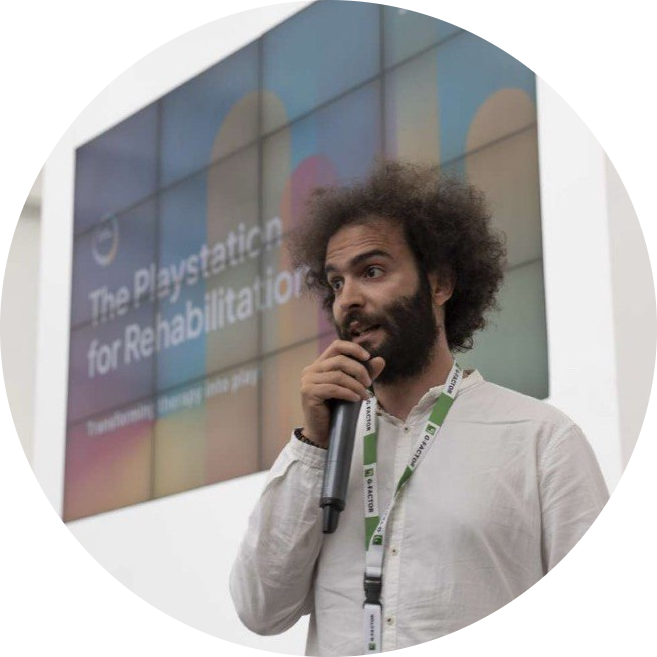
\includegraphics[width=2.8cm]{Pictures/Giovanni_pitch}
\end{minipage}
\vspace{0.1em}
}

\makeatletter
% the sender details are already in \clheader, so skip moderncv's own block
\@detailsfalse
% closing phrase, signature, name
\renewcommand*{\makeletterclosing}{%
  \@closing\\[0.6em]%
  
\includegraphics[height=1.2cm]{Pictures/sign_gt.jpg}\\[0.2em]%
  {\bfseries\@firstname~\@lastname}}
\makeatother


\begin{document}

\clheader{R\&D Engineer, PhD Candidate | Human Behaviour \& Data Analysis}

\recipient{Recruitment Team}{Network and Behavioural Scientist}
\opening{Dear Hiring Team,}
\closing{Yours faithfully,}
\makelettertitle

I am applying for the Network and Behavioural Scientist position. I am an R\&D engineer and PhD candidate with more than five years of applied research at CNR-STIIMA, the Italian National Research Council, studying how people behave and respond to feedback, and I would like to apply that work to human behaviour at scale.

My research is experimental and data-driven. For my PhD at the University of Bologna I developed OmniTrack, an IoT-based multimodal navigation system, and ran navigation experiments with 16 blind participants, collecting position and IMU data and analysing in Python how they respond to multimodal feedback. Two research stays shaped this work: sensory navigation and experimental psychology at Utrecht University, and feedback algorithms and behaviour analysis at Toyo University in Tokyo.

I am used to developing methods rather than only applying them. Where no existing tool fitted, I built the sensing platform, the feedback algorithm and the analysis pipeline myself, and validated them with real users. I have also built embedded machine-learning classifiers with TensorFlow Lite, and I have seen research become a working system: PhiCube, a rehabilitation device I co-invented, is now in two ongoing multicentre studies with 134 patients through Rehabilia Technologies, the company I co-founded.

I come to network science from the behavioural side: my data so far are trajectories and sensor signals rather than social graphs. What I bring is experimental design, analysis of noisy real-world behavioural data in Python and experience validating new methods with real people, and I am keen to extend this to network methods together with your team.

I would welcome the chance to discuss the role further.

\makeletterclosing

\end{document}
